\appendix
\section{Abschwächung des Lasers}
\label{sec:laser}
In der folgenden Rechnung wird berechnet, wie stark das Laserlicht abgeschwächt
werden muss, damit mit \SI{99,9}{\percent}iger Wahrscheinlichkeit nur ein
einziges Photon pro Puls an der Photodiode ankommt. Dafür wird verwendet, dass
die Photonenzahl beim Laser einer Poisson-Statistik unterliegt. Zunächst muss
berechnet werden, wie viele Photonen sich in einem Puls befinden (Photonenzahl
$N_P$), und anschließend kann bestimmt werden, um welchen Faktor die Intensität
verringert werden muss, um die genannte Wahrscheinlichkeit zu erreichen, nur ein
einziges Photon zu detektieren.
\begin{eqnarray}
E_{\mathrm{Puls}} &=& \SI{50}{mW}\cdot\SI{10}{ns} = \SI{50e-12}{J}\\
E_{\mathrm{Photon}} &=& hν = h\frac{c}{λ}\\
N_P &=& \frac{E_{\mathrm{Puls}}}{E_{\mathrm{Puls}}} = \SI{1,6e8}{}
\end{eqnarray}
Dies entspricht dem Erwartungswert λ der Photonenanzahl.
\begin{eqnarray}
P_λ(X=k) &=& \frac{λ^k}{k!}\mathrm{e}^{-λ}\\
\rightarrow P_{cλ}(1) &=& cλ\cdot\mathrm{e}^{-cλ} = \SI{0.999}{}
\end{eqnarray}
Hierbei ist $c$ eine Konstante, die beschreibt, welcher Anteil des Lichts die
Filter passieren soll. Diese Gleichung kann numerisch gelöst werden, wobei sich
hier das folgende für $c$ ergibt:
\begin{equation}
c = \SI{1.2e6}{}
\end{equation}
Wenn also die Filter so gewählt werden, dass die Intensität um einen Faktor von
ca. $10^6$ verringert wird, kann man davon ausgehen, dass nur ein Photon eines
Pulses den Detektor erreicht.

\section{Wahl der Polarisation}
\label{sec:zirkular}
Hier wird gezeigt, dass es möglich ist, als mögliche Polarisationszustände eine
horizontale, vertikale, rechts- und linkszirkulare Polarisation zu verwenden.
Dafür muss gezeigt werden, dass die zur gleichen Basis gehörenden Zustände
orthogonal zueinander sind, während die Zustände, die zu unterschiedlichen
Basen gehören, nicht orthogonal zueinander sein sollen.
\begin{eqnarray}
| \circlearrowright \rangle &=& \frac{1}{\sqrt{2}}(|\rightarrow\rangle +
i|\uparrow\rangle)\\
| \circlearrowleft \rangle &=& \frac{1}{\sqrt{2}}(|\rightarrow\rangle -
i|\uparrow\rangle)\\
\langle\uparrow|\uparrow\rangle &=& 1\\
\langle\uparrow|\rightarrow\rangle &=& 0\\
\langle\circlearrowleft|\circlearrowleft \rangle &=& 1\\
\langle\circlearrowleft|\circlearrowright \rangle &=& 0\\
|\langle\uparrow|\circlearrowleft \rangle| &=&
\left|\frac{1}{\sqrt{2}}\langle\uparrow|(|\rightarrow\rangle -
i|\uparrow\rangle\right|\\
 &=& \frac{1}{\sqrt{2}}\\
|\langle\uparrow|\circlearrowright \rangle| &=& \frac{1}{\sqrt{2}}\\
|\langle\rightarrow|\circlearrowleft \rangle| &=&
\left|\frac{1}{\sqrt{2}}\langle\rightarrow|(|\rightarrow\rangle -
i|\uparrow\rangle\right|\\
 &=& \frac{1}{\sqrt{2}}\\
|\langle\rightarrow|\circlearrowright \rangle| &=& \frac{1}{\sqrt{2}}
\end{eqnarray}
Man kann erkennen, dass die Skalarprodukte der beiden zur jeweils gleichen
Basis gehörenden Polarisationen für orthogonal zueinander stehende
Polarisationen null werden, was zu einer deterministischen Messung bei der Wahl
gleicher Basen von Alice und Bob führt. Andererseits sind die Skalarprodukte
von zu unterschiedlichen Basen gehörenden Polarisationen vom Betrage her immer
$1/\sqrt{2}$, sodass gar keine Aussage über den Polarisationszustand getroffen
werden kann, wenn die beiden unterschiedliche Basen verwenden. Somit ist
gezeigt, dass die in unserem Experiment getroffene Wahl einer orthogonalen,
linear-polarisierten und einer zirkular-polarisierten Basis für den Zweck der
quantenkryptographischen Schlüsselübertragung geeignet ist.

\onecolumn
\section{Messprotokoll}
\label{sec:protokoll}
\begin{figure}[!ht]
        \centering
        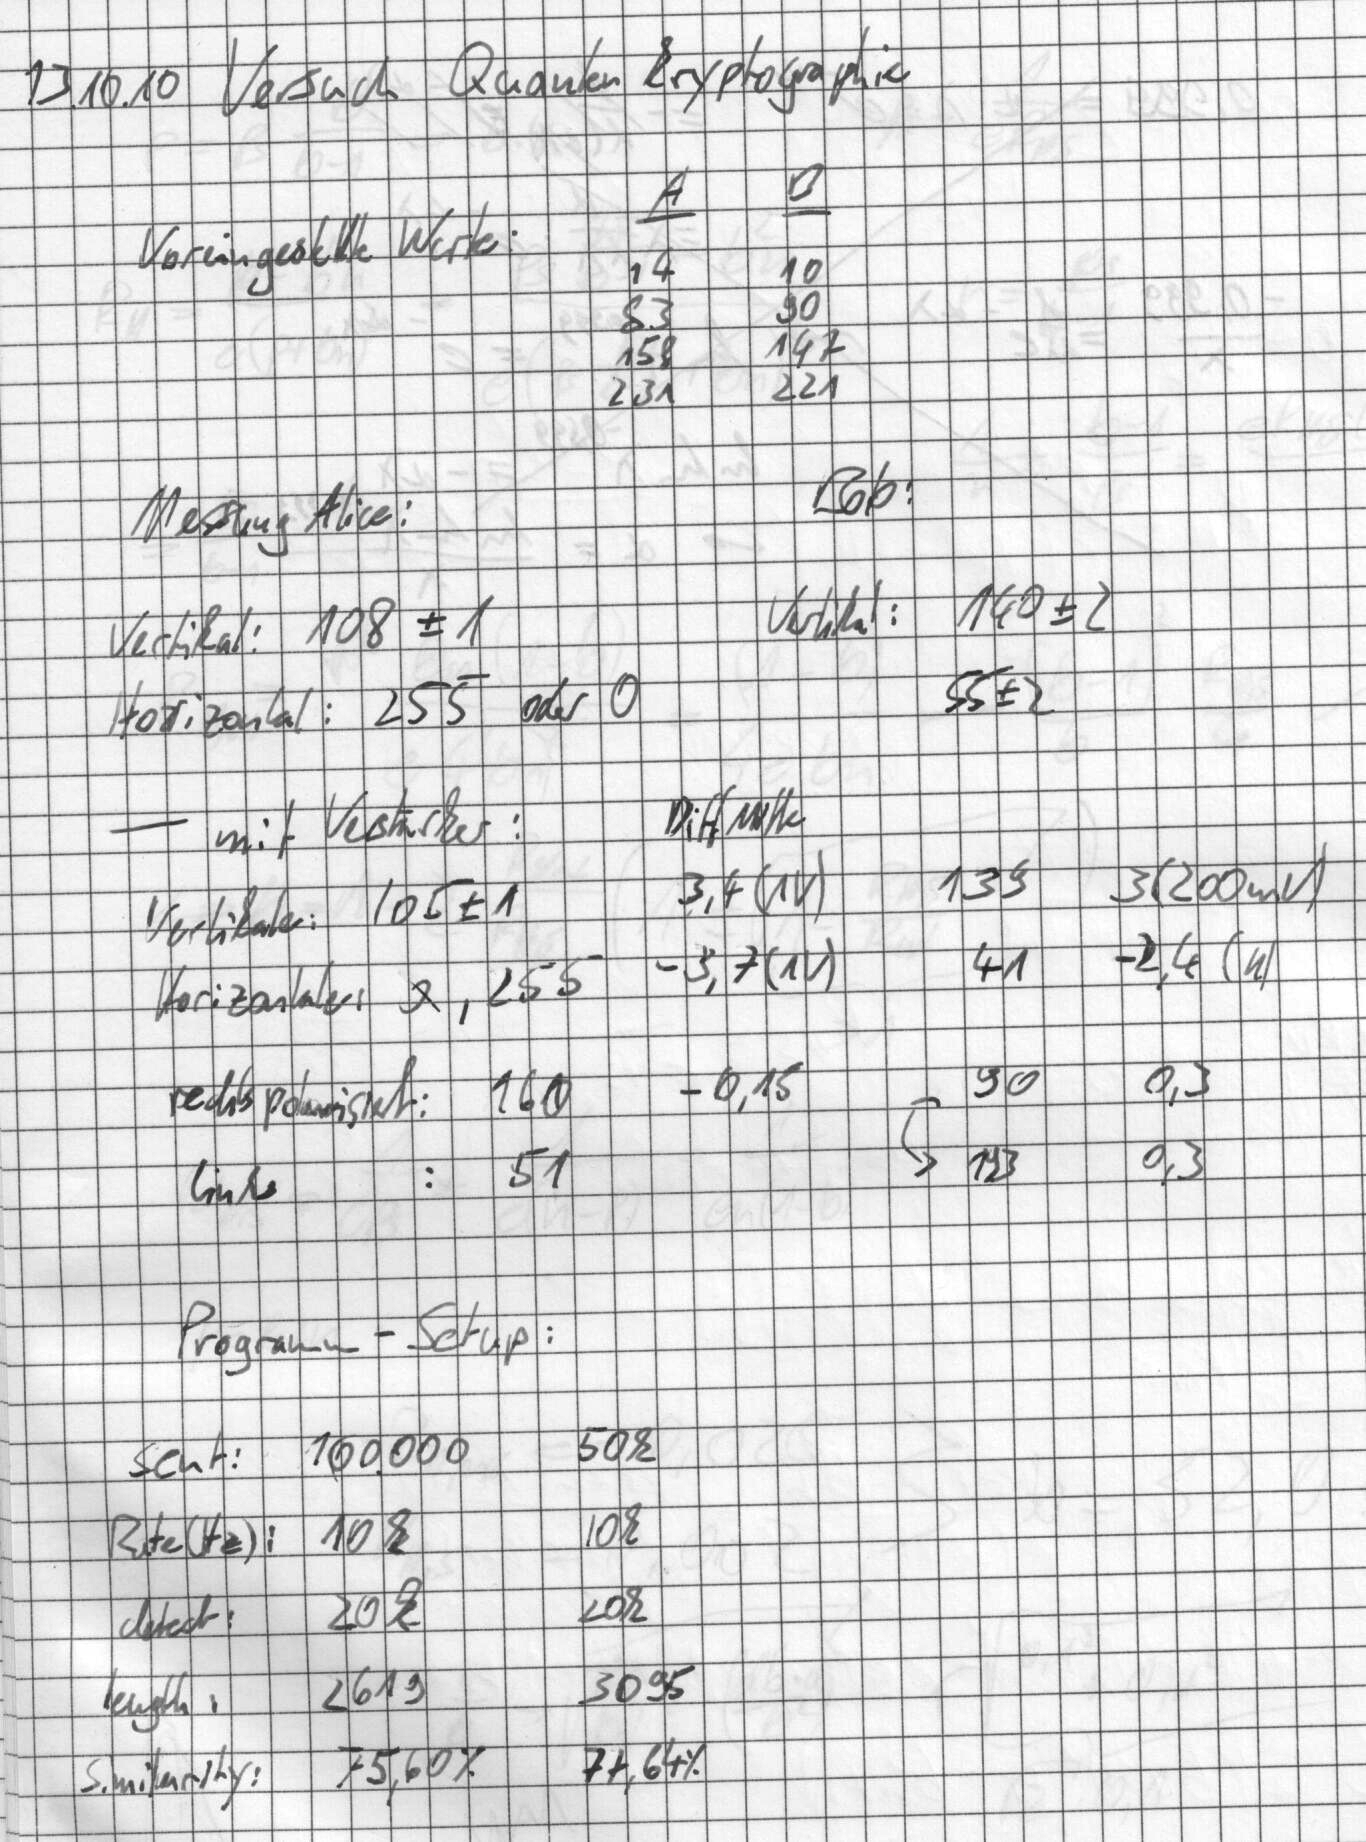
\includegraphics[page=1,width=.88\textwidth,keepaspectratio]{../data/messprotokoll}
%         \caption{Messprotokoll}
        \label{fig:protokoll}
\end{figure}

\section{Messwerttabellen}
\subsection{Similarity}
\label{sec:messwerttabellen}

\label{Schlüssellängen}
\label{sec:keylength}